\chapter{Advanced Predictive Modelling and Ensemble Learning (Unit 5)}

\section{Overview of Allotted Unit 5 Topics}
Group 10's PBL III topic is \textbf{Diabetes Prediction}: \emph{develop an intelligent diabetes prediction model using
patient health records, and investigate how effective different ensemble classifiers are at identifying individuals at
risk of diabetes.} The review requires at least three ensemble algorithms, a comparison against a baseline (Logistic
Regression or Decision Tree), and evaluation with F1-score and ROC-AUC.

\textbf{Ensemble learning} combines $M$ base learners $h_1,\dots,h_M$ into a stronger predictor
$H(\mathbf x)=\sum_m w_m h_m(\mathbf x)$. For averaged models, the error decomposes into bias and variance. Averaging
$M$ learners, each with variance $\sigma^2$ and pairwise correlation $\rho$, gives
\begin{equation}
\operatorname{Var}\!\Big[\tfrac{1}{M}\textstyle\sum_m h_m\Big]=\rho\,\sigma^2+\frac{1-\rho}{M}\,\sigma^2 ,
\label{eq:var}
\end{equation}
so \textbf{bagging} methods reduce variance by averaging many decorrelated trees, while \textbf{boosting} methods reduce
bias by adding learners sequentially, each correcting its predecessors' errors \cite{esl}. This chapter implements
\textbf{ten ensembles} from three families and compares them with two single-model baselines:
\begin{itemize}
\item \textbf{Bagging family:} Bagging \cite{breiman96}, Random Forest \cite{breiman01} and Extra Trees \cite{geurts}.
\item \textbf{Boosting family:} AdaBoost \cite{freund}, Gradient Boosting \cite{friedman}, XGBoost \cite{xgboost},
LightGBM \cite{lightgbm} and CatBoost \cite{catboost}.
\item \textbf{Meta-ensembles:} Soft Voting and Stacking \cite{wolpert} over the four strongest learners.
\item \textbf{Baselines:} Logistic Regression and a single Decision Tree (CART).
\end{itemize}

\section{Dataset Description and Preprocessing}
A new dataset is used for Unit 5: the \textbf{Diabetes Prediction Dataset} \cite{diabdata}. It contains
\dbRowsRaw{} electronic patient records with eight predictors and a binary target (diabetes yes/no).

\begin{table}[H]
\centering
\caption{Attributes of the Diabetes Prediction Dataset}
\label{tab:dbattr}
\renewcommand{\arraystretch}{1.2}
\begin{tabularx}{\linewidth}{@{}l l >{\raggedright\arraybackslash}X@{}}
\toprule
\textbf{Attribute} & \textbf{Type} & \textbf{Description / range} \\
\midrule
gender & categorical & Female, Male (and 18 records ``Other'') \\
age & continuous & 0.08–80 years \\
hypertension & binary & 1 if the patient has hypertension (7.5\%) \\
heart\_disease & binary & 1 if the patient has heart disease (3.9\%) \\
smoking\_history & categorical & never, former, current, not current, ever, No Info \\
bmi & continuous & body-mass index, 10.0–95.7 kg/m$^2$ \\
HbA1c\_level & continuous & glycated haemoglobin, 3.5–9.0\% (average blood sugar over 2–3 months) \\
blood\_glucose\_level & continuous & blood glucose at the time of measurement, 80–300 mg/dL \\
\midrule
\textbf{diabetes} & \textbf{binary target} & 1 = diabetic (8.5\% before cleaning) \\
\bottomrule
\end{tabularx}
\end{table}

\textbf{Relevance.} These are exactly the routinely collected variables a clinician sees: demographics, comorbidities,
lifestyle, and the two laboratory markers used for diagnosis \cite{ada}. The dataset is large enough
(\dbRowsRaw{} records) for a reliable comparison of many ensembles with cross-validation.

\textbf{Preprocessing.}
\begin{enumerate}
\item \textbf{Duplicates:} \dbDup{} exact duplicate records were removed. Otherwise identical rows could appear in both
the training and test sets and inflate the scores.
\item \textbf{Rare category:} gender ``Other'' (18 records) was dropped, since it is too rare to learn from. This leaves
\textbf{\dbRowsClean{} patients}, with a diabetes prevalence of \dbPrev.
\item \textbf{Missing information:} there are no null values, but smoking history is ``No Info'' for about 36\% of
patients. This is kept as its own category, because whether smoking was recorded is itself informative, and imputing
it would invent information.
\item \textbf{Outliers:} all values are clinically plausible, so none were removed; high values are genuine high-risk
patients.
\item \textbf{Encoding and scaling:} one-hot encoding for gender and smoking history, and standardisation of numeric
features, inside a scikit-learn \texttt{Pipeline}. Standardisation is needed by Logistic Regression and harmless for
trees.
\item \textbf{Split:} a stratified 80/20 split into \dbTrain{} training and \dbTest{} test patients, keeping the
prevalence in both sets. The test set is used once. All model comparisons use \textbf{5-fold stratified
cross-validation} on the training set.
\end{enumerate}
\begin{pycode}
df = df_raw.drop_duplicates()
df = df[df.gender != "Other"].reset_index(drop=True)
pre = ColumnTransformer([("num", StandardScaler(), ["age", "bmi", "HbA1c_level", "blood_glucose_level",
                                                    "hypertension", "heart_disease"]),
                         ("cat", OneHotEncoder(handle_unknown="ignore"), ["gender", "smoking_history"])])
X_train, X_test, y_train, y_test = train_test_split(X, y, test_size=0.2, stratify=y, random_state=42)
cv = StratifiedKFold(n_splits=5, shuffle=True, random_state=42)
\end{pycode}

\section{EDA and Feature Analysis}
\begin{figure}[H]
\centering
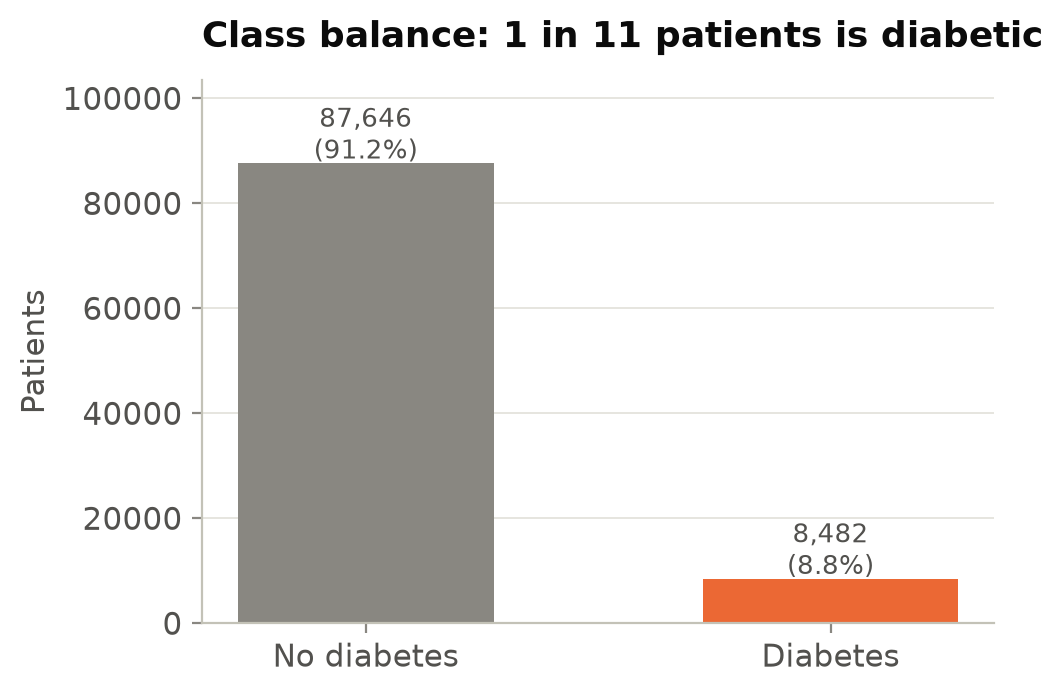
\includegraphics[width=0.40\linewidth]{db_class_balance.png}\hfill
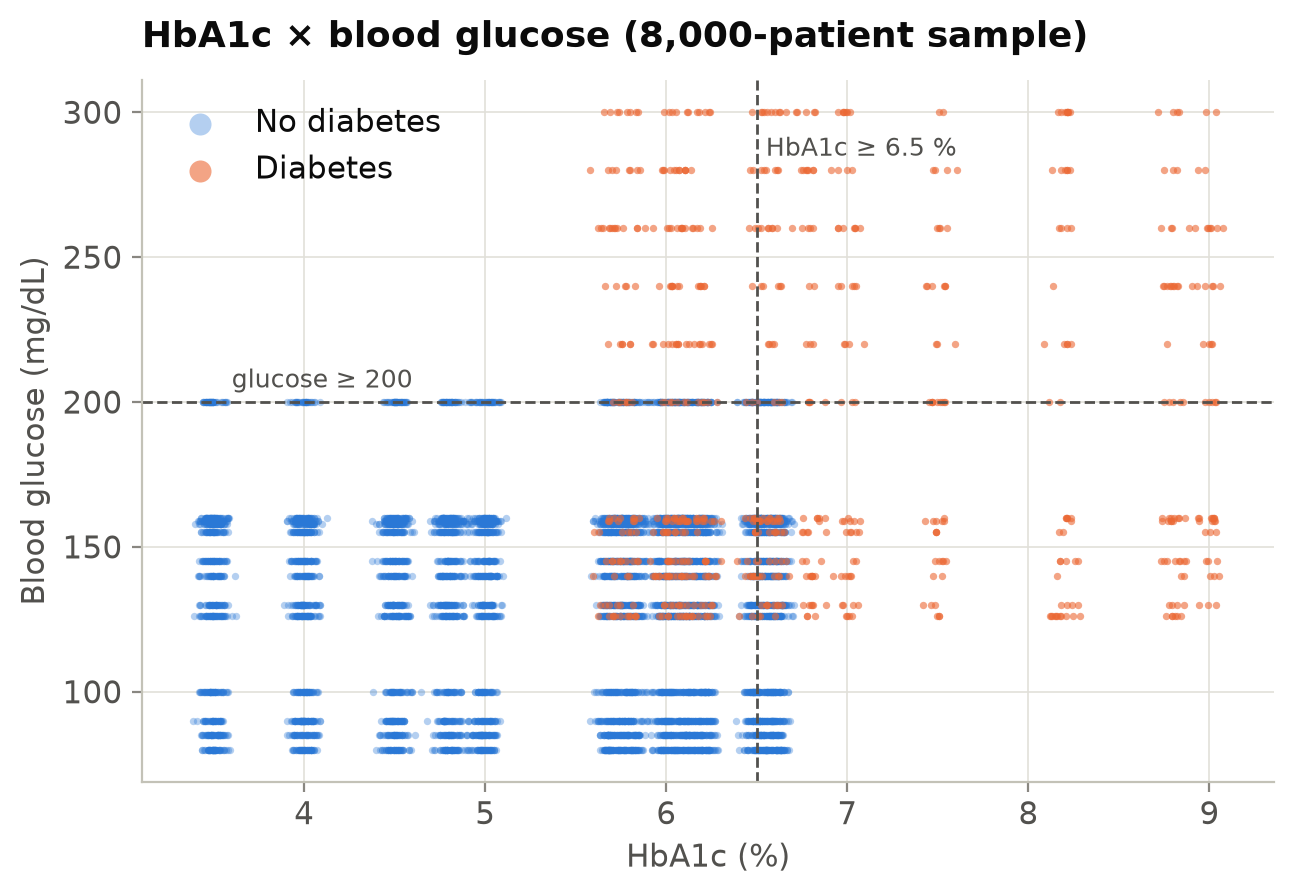
\includegraphics[width=0.56\linewidth]{db_hba1c_glucose.png}
\caption{Class balance (left) and HbA1c against blood glucose for 8,000 patients (right)}
\label{fig:dbbal}
\end{figure}
\textbf{Interpretation (Figure~\ref{fig:dbbal}).} Only \dbPrev{} of patients are diabetic, so the target is imbalanced. A
model that always predicts ``no diabetes'' would be 91\% accurate yet useless. We therefore judge models by
\textbf{F1-score, ROC-AUC and PR-AUC}, not accuracy. HbA1c and glucose are recorded at a small set of discrete levels.
Every patient with HbA1c $>$ 6.6\% or glucose $>$ 200 mg/dL is diabetic. These patients make up \dbRuleShare{} of the
data and account for \dbRuleCapture{} (two-thirds) of all diabetics; they are easy to classify. The remaining third of
diabetics have laboratory values inside the normal range, and these \emph{hard cases} are where a model must combine
age, BMI, comorbidities and the laboratory values.

\begin{figure}[H]
\centering
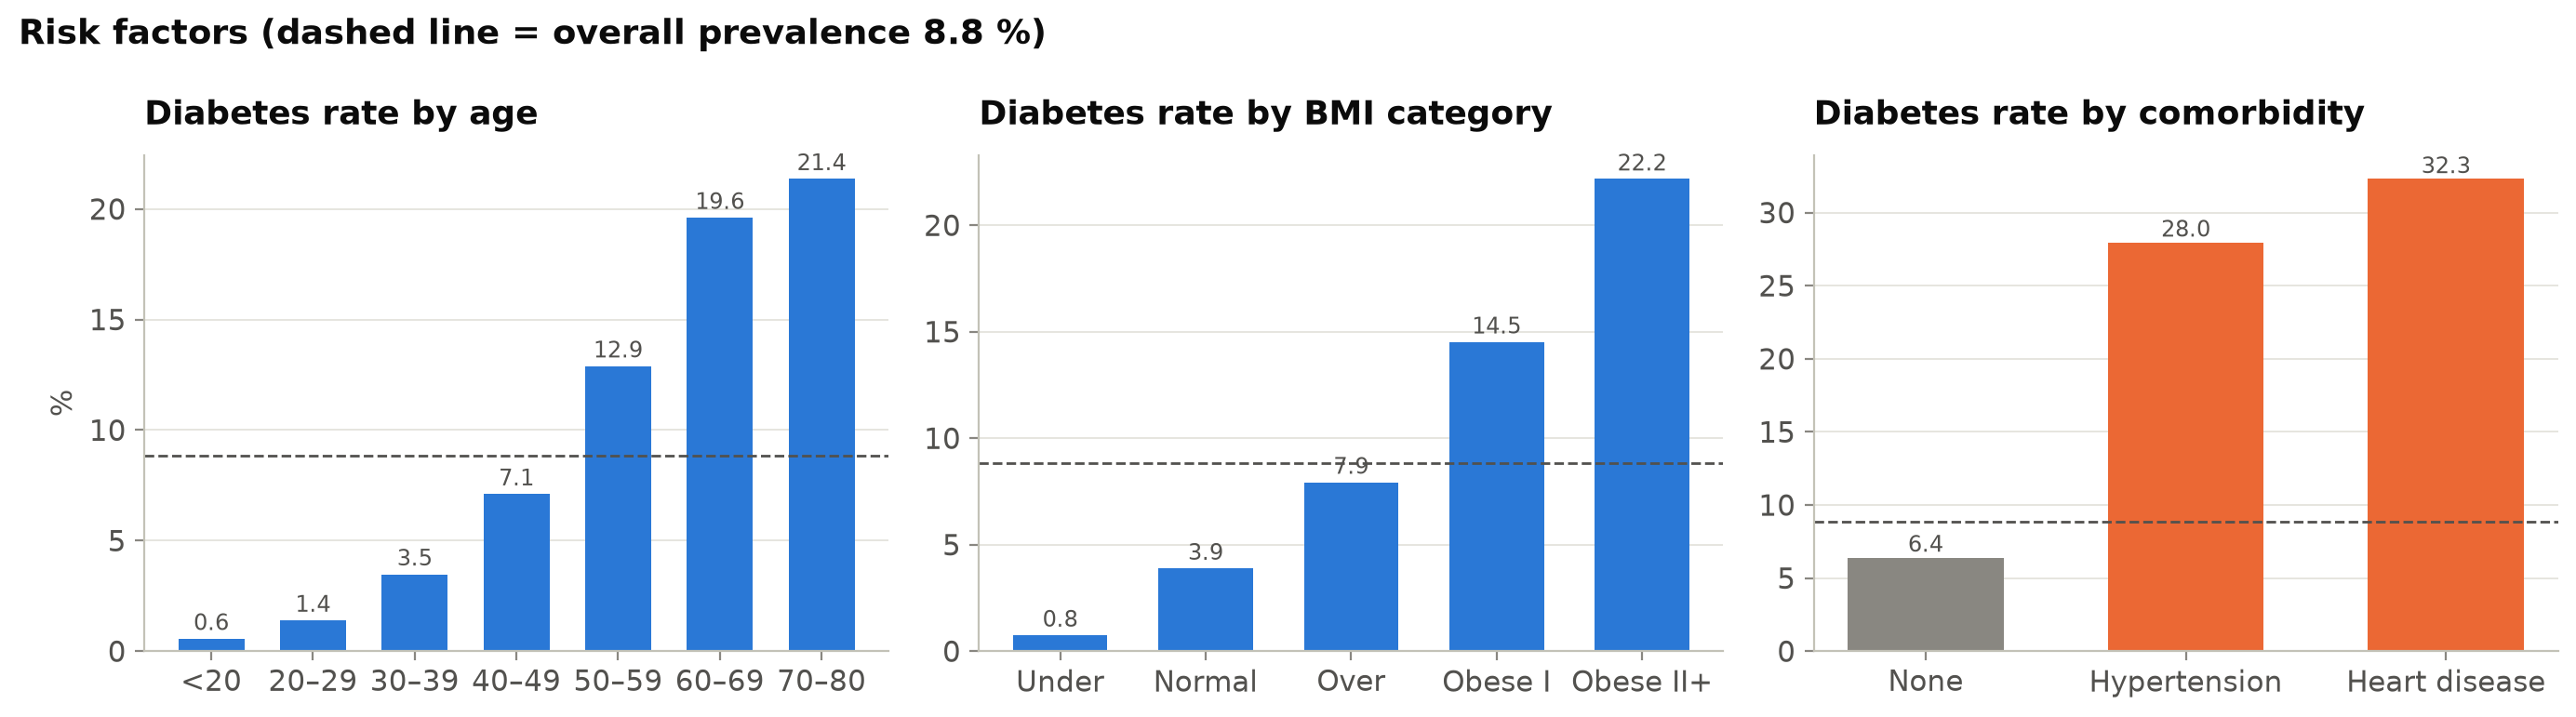
\includegraphics[width=\linewidth]{db_risk_factors.png}
\caption{Diabetes rate by age group, BMI category and comorbidity (dashed line = overall prevalence)}
\label{fig:dbrisk}
\end{figure}
\textbf{Interpretation (Figure~\ref{fig:dbrisk}).} Risk rises steeply and non-linearly with age, from 0.6\% under 20
to 21.4\% at 70–80. It also rises with BMI, from 3.9\% at normal weight to 22.2\% in severe obesity, and with
comorbidity: 28.0\% with hypertension and 32.3\% with heart disease, against 6.4\% without either. These monotone but
non-linear, interacting effects are what tree ensembles capture without manual feature engineering.

\begin{figure}[H]
\centering
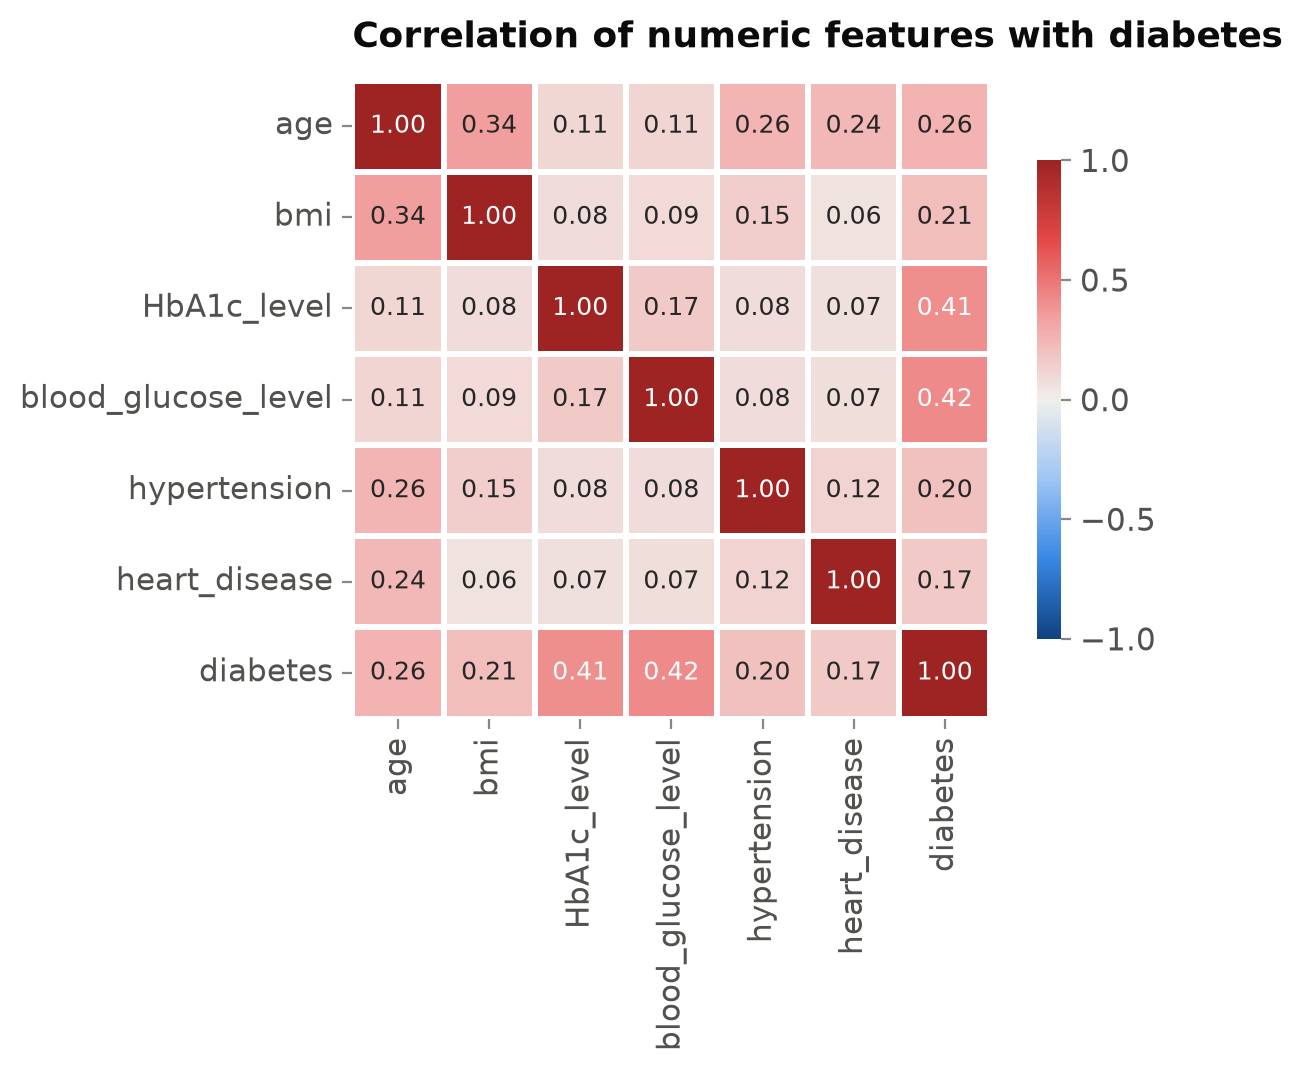
\includegraphics[width=0.49\linewidth]{db_correlation.png}\hfill
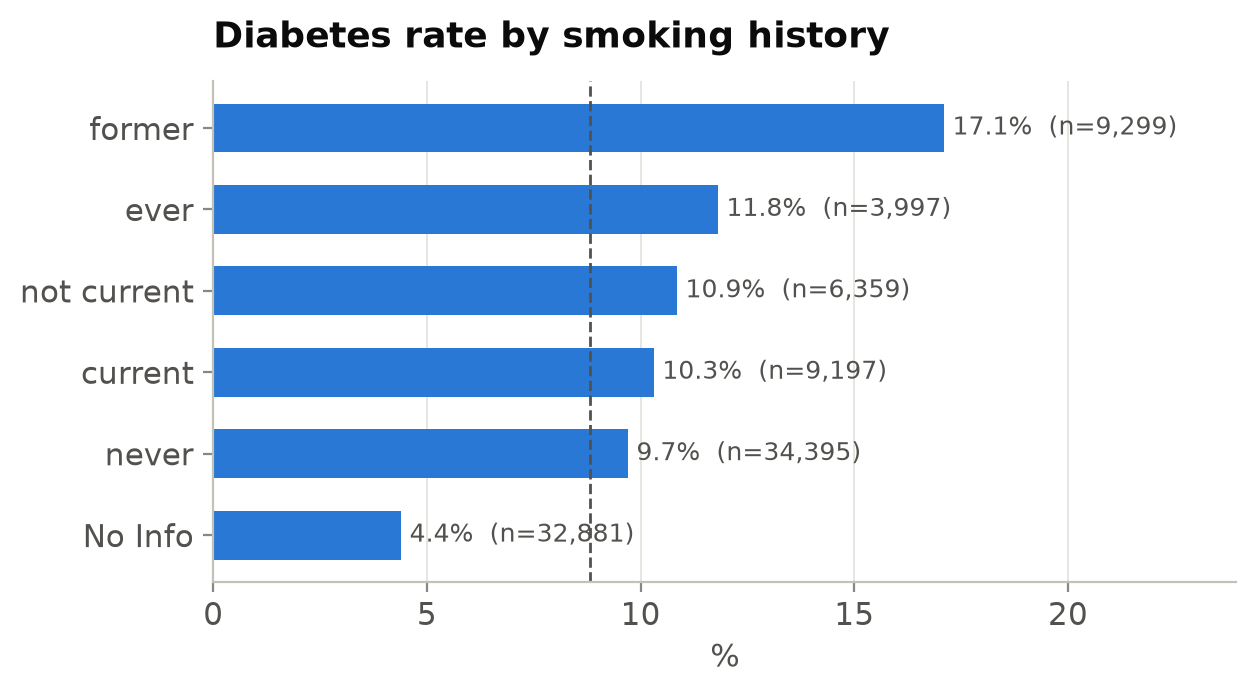
\includegraphics[width=0.49\linewidth]{db_smoking.png}
\caption{Correlation of numeric features with diabetes (left); diabetes rate by smoking history (right)}
\label{fig:dbcorr}
\end{figure}
\textbf{Interpretation (Figure~\ref{fig:dbcorr}).} Blood glucose (0.42) and HbA1c (0.41) are the strongest single
correlates, followed by age (0.26), BMI (0.21), hypertension (0.20) and heart disease (0.17). Correlations among the
predictors are weak (all $\le$0.34), so multicollinearity is not a concern. Former smokers have the highest rate
(17.1\%). Patients with ``No Info'' have the lowest (4.4\%), largely because this group contains many children, which
confirms that the missingness is informative and should be kept as a category.

\begin{figure}[H]
\centering
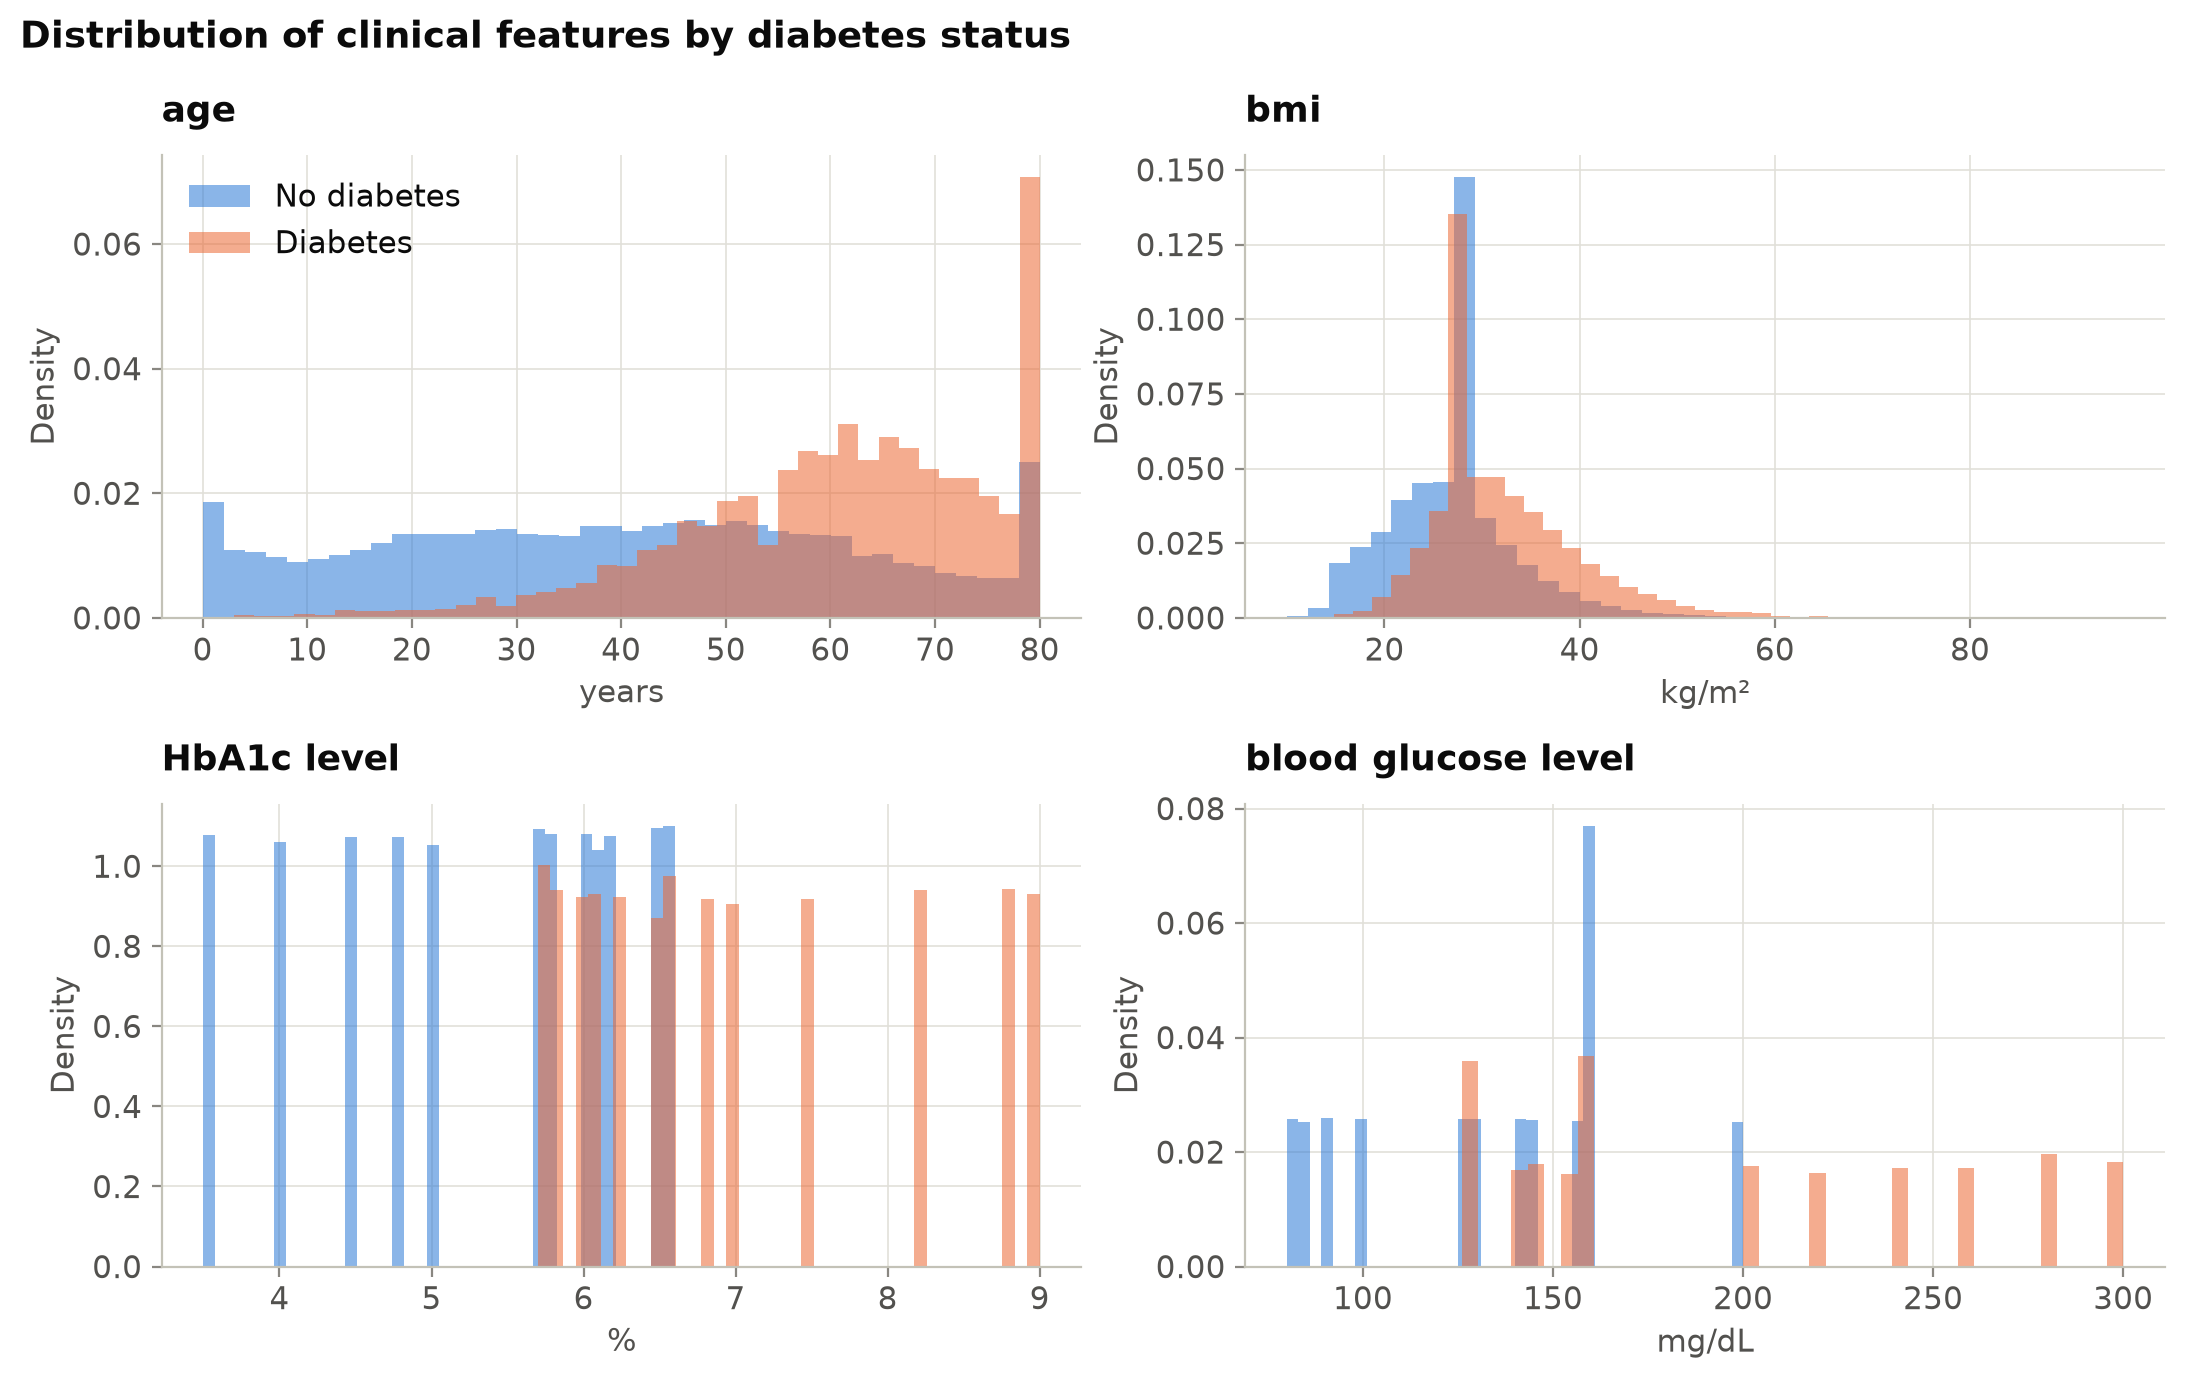
\includegraphics[width=\linewidth]{db_feature_distributions.png}
\caption{Distribution of the four clinical features by diabetes status}
\label{fig:dbdist}
\end{figure}
\textbf{Interpretation (Figure~\ref{fig:dbdist}).} Diabetic patients are older and have higher BMI. Their HbA1c and
glucose distributions extend into ranges (HbA1c 6.8–9\%, glucose 220–300) that never occur in non-diabetics, while
overlapping substantially with non-diabetics at lower levels.

\section{Proposed Workflow / Architecture}
\begin{figure}[H]
\centering
\resizebox{\linewidth}{!}{%
\begin{tikzpicture}[font=\small,
  box/.style={draw=navy, fill=lightblue, rounded corners=3pt, minimum height=1.35cm, text width=3.0cm, align=center},
  hl/.style={box, fill=lightorange, draw=accent}, gr/.style={box, fill=green!8, draw=green!50!black},
  arr/.style={-{Stealth[length=2.5mm]}, thick, navy}, bus/.style={thick, navy}]
\node[box] (a) at (0,0) {Patient records (100,000)};
\node[box] (b) at (3.8,0) {Clean: duplicates, rare category};
\node[box] (c) at (7.6,0) {Stratified 80/20 split};
\node[box] (d) at (11.4,0) {Pipeline: one-hot + scaling};
\node[gr] (e) at (0,-2.6) {Baselines: Logistic Regression, Decision Tree};
\node[hl] (f) at (3.8,-2.6) {Bagging: Bagging, Random Forest, Extra Trees};
\node[hl] (g) at (7.6,-2.6) {Boosting: AdaBoost, GB, XGBoost, LightGBM, CatBoost};
\node[hl] (h) at (11.4,-2.6) {Meta-ensembles: Soft Voting, Stacking};
\node[box] (i) at (0,-5.2) {5-fold stratified CV (F1, ROC-AUC, PR-AUC)};
\node[box] (j) at (3.8,-5.2) {Final model = best CV F1};
\node[box] (k) at (7.6,-5.2) {LightGBM tuning; F1-optimal threshold (OOF)};
\node[box] (l) at (11.4,-5.2) {Test set: metrics, McNemar, SHAP};
\draw[arr] (a)--(b); \draw[arr] (b)--(c); \draw[arr] (c)--(d);
\coordinate (t1) at (0,-1.3); \coordinate (t2) at (0,-3.9);
\draw[bus] (d.south) -- (d.south |- t1);
\draw[bus] (e.north |- t1) -- (h.north |- t1);
\foreach \n in {e,f,g,h} \draw[arr] (\n.north |- t1) -- (\n.north);
\foreach \n in {e,f,g,h} \draw[bus] (\n.south) -- (\n.south |- t2);
\draw[bus] (e.south |- t2) -- (h.south |- t2);
\draw[arr] (e.south |- t2) -- (i.north);
\draw[arr] (i)--(j); \draw[arr] (j)--(k); \draw[arr] (k)--(l);
\end{tikzpicture}}
\caption{Unit 5 workflow: preprocessing, 2 baselines and 10 ensembles, CV-based selection, tuning, threshold optimisation and test evaluation}
\label{fig:wf5}
\end{figure}
\textbf{Stages.} (1) The patient records are cleaned and split (stratified) before any fitting. (2) Every model is a
pipeline of the same preprocessing plus the classifier, so encoding and scaling never see validation or test data.
(3) The twelve models are compared with identical 5-fold stratified CV. (4) The final model is the one with the highest CV F1, chosen without
looking at the test set; LightGBM is additionally tuned by randomised search. (5) Because the classes are imbalanced, the decision threshold is chosen to maximise F1 on
\emph{out-of-fold} training predictions. (6) The held-out test set is used once, for the final metrics, McNemar's
significance test and SHAP interpretation.

\section{Algorithm Theory and Mathematical Formulation}
\subsection{Baselines}
\textbf{Logistic Regression} models $P(y=1\mid\mathbf x)=\sigma(\mathbf w^\top\mathbf x+b)$ and minimises the log-loss
(Chapter 2). It is linear in the features, so it cannot represent the steep, interacting thresholds seen in the EDA.
A \textbf{Decision Tree (CART)} recursively chooses the split that maximises the decrease in Gini impurity
$G=1-\sum_k p_k^2$. A fully grown tree has low bias but very high variance.

\subsection{Bagging family}
\textbf{Bagging} trains $M$ trees on bootstrap samples (drawn with replacement) and averages their predicted
probabilities, $\hat p(\mathbf x)=\frac1M\sum_m h_m(\mathbf x)$. By Equation~(\ref{eq:var}), averaging reduces variance
as long as the trees are not perfectly correlated. \textbf{Random Forest} decorrelates the trees further by considering
only a random subset of features ($\sqrt d$) at each split, which lowers $\rho$. \textbf{Extra Trees} also draws the
split thresholds at random, trading a little bias for further variance reduction.
\emph{Settings:} 200 bagged trees; 300 trees with \texttt{min\_samples\_leaf}=2 for RF and Extra Trees.

\subsection{Boosting family}
\textbf{AdaBoost} fits weak learners (decision stumps) sequentially. After round $m$, with weighted error
$\varepsilon_m$, the learner receives weight $\alpha_m=\tfrac12\ln\frac{1-\varepsilon_m}{\varepsilon_m}$, and the
misclassified samples are up-weighted, $w_i\leftarrow w_i\,e^{\alpha_m\,\mathbb 1[h_m(\mathbf x_i)\ne y_i]}$.
The final model is $H(\mathbf x)=\operatorname{sign}\sum_m\alpha_m h_m(\mathbf x)$.
\emph{Settings:} 300 estimators, learning rate 0.5.

\textbf{Gradient Boosting} builds an additive model $F_m(\mathbf x)=F_{m-1}(\mathbf x)+\eta\,h_m(\mathbf x)$, where each
tree $h_m$ is fitted to the negative gradient of the log-loss, the pseudo-residuals $r_{im}=y_i-p_{m-1}(\mathbf x_i)$.
\emph{Settings:} 300 trees of depth 3, learning rate $\eta=0.1$.

\textbf{XGBoost} minimises a regularised second-order approximation of the loss. For a tree with leaf weights $w_j$ and
gradient/Hessian sums $G_j,H_j$, the optimal leaf weight and the gain of a split are
\begin{equation}
w_j^\star=-\frac{G_j}{H_j+\lambda},\qquad
\text{Gain}=\tfrac12\Big[\frac{G_L^2}{H_L+\lambda}+\frac{G_R^2}{H_R+\lambda}-\frac{(G_L+G_R)^2}{H_L+H_R+\lambda}\Big]-\gamma .
\end{equation}
\textbf{LightGBM} uses the same objective with histogram-based split finding and \emph{leaf-wise} tree growth, which is
much faster. \textbf{CatBoost} uses \emph{ordered boosting} and symmetric (oblivious) trees, which reduces prediction
shift and over-fitting. \emph{Settings:} XGBoost and LightGBM with 400 trees, learning rate 0.05 and 0.9 row/column
subsampling; CatBoost with 500 iterations, depth 6, learning rate 0.08.

\subsection{Meta-ensembles}
\textbf{Soft Voting} averages the predicted probabilities of Random Forest, XGBoost, LightGBM and CatBoost.
\textbf{Stacking} trains a logistic-regression \emph{meta-learner} on the out-of-fold probabilities of the same four
base models (5-fold internal CV), learning how much to trust each one:
$\hat p(\mathbf x)=\sigma\big(\beta_0+\sum_{m}\beta_m\,\hat p_m^{\text{OOF}}(\mathbf x)\big)$.

\subsection{Model selection, tuning and threshold}
\begin{itemize}
\item \textbf{Cross-validation:} all twelve models use the same 5 stratified folds of the training set, scored on
accuracy, precision, recall, F1, ROC-AUC and PR-AUC.
\item \textbf{Hyperparameter tuning:} LightGBM was tuned with \texttt{RandomizedSearchCV}: 40 random configurations
$\times$ 5 folds, scored on PR-AUC, which focuses on the rare positive class. The search covered the number of trees,
learning rate, leaves, depth, minimum child samples, subsampling and $L_1$/$L_2$ regularisation (best CV PR-AUC
\dbTuneAp{}, \dbTuneSec{} minutes).
\item \textbf{Threshold:} the decision threshold $t^\star=\arg\max_t F_1(t)$ was chosen on 5-fold \emph{out-of-fold}
predictions of the training set and applied unchanged to the test set.
\item \textbf{Significance:} a paired $t$-test on the per-fold F1 scores against Logistic Regression, and McNemar's
test \cite{mcnemar} on test-set predictions,
$\chi^2=\frac{(|n_{01}-n_{10}|-1)^2}{n_{01}+n_{10}}$, where $n_{01}$ and $n_{10}$ count the patients that only one of
the two models classifies correctly.
\end{itemize}

\begin{table}[H]
\centering
\caption{Tuned LightGBM hyperparameters (randomised search, 40 $\times$ 5-fold CV, PR-AUC)}
\label{tab:tuned}
\begin{tabular}{@{}ll@{}}
\toprule
\textbf{Hyperparameter} & \textbf{Selected value} \\
\midrule
\dbTunedRows
\bottomrule
\end{tabular}
\end{table}

\section{Results and Performance Evaluation}
\begin{table}[H]
\centering
\caption{5-fold stratified cross-validation on the training set (sorted by mean F1)}
\label{tab:dbcv}
\resizebox{\linewidth}{!}{%
\begin{tabular}{@{}llcccccc@{}}
\toprule
\textbf{Model} & \textbf{Family} & \textbf{F1 (mean $\pm$ sd)} & \textbf{ROC-AUC} & \textbf{PR-AUC} & \textbf{Precision} & \textbf{Recall} & \textbf{CV time (s)} \\
\midrule
\dbCvRows
\bottomrule
\end{tabular}}
\end{table}

\begin{figure}[H]
\centering
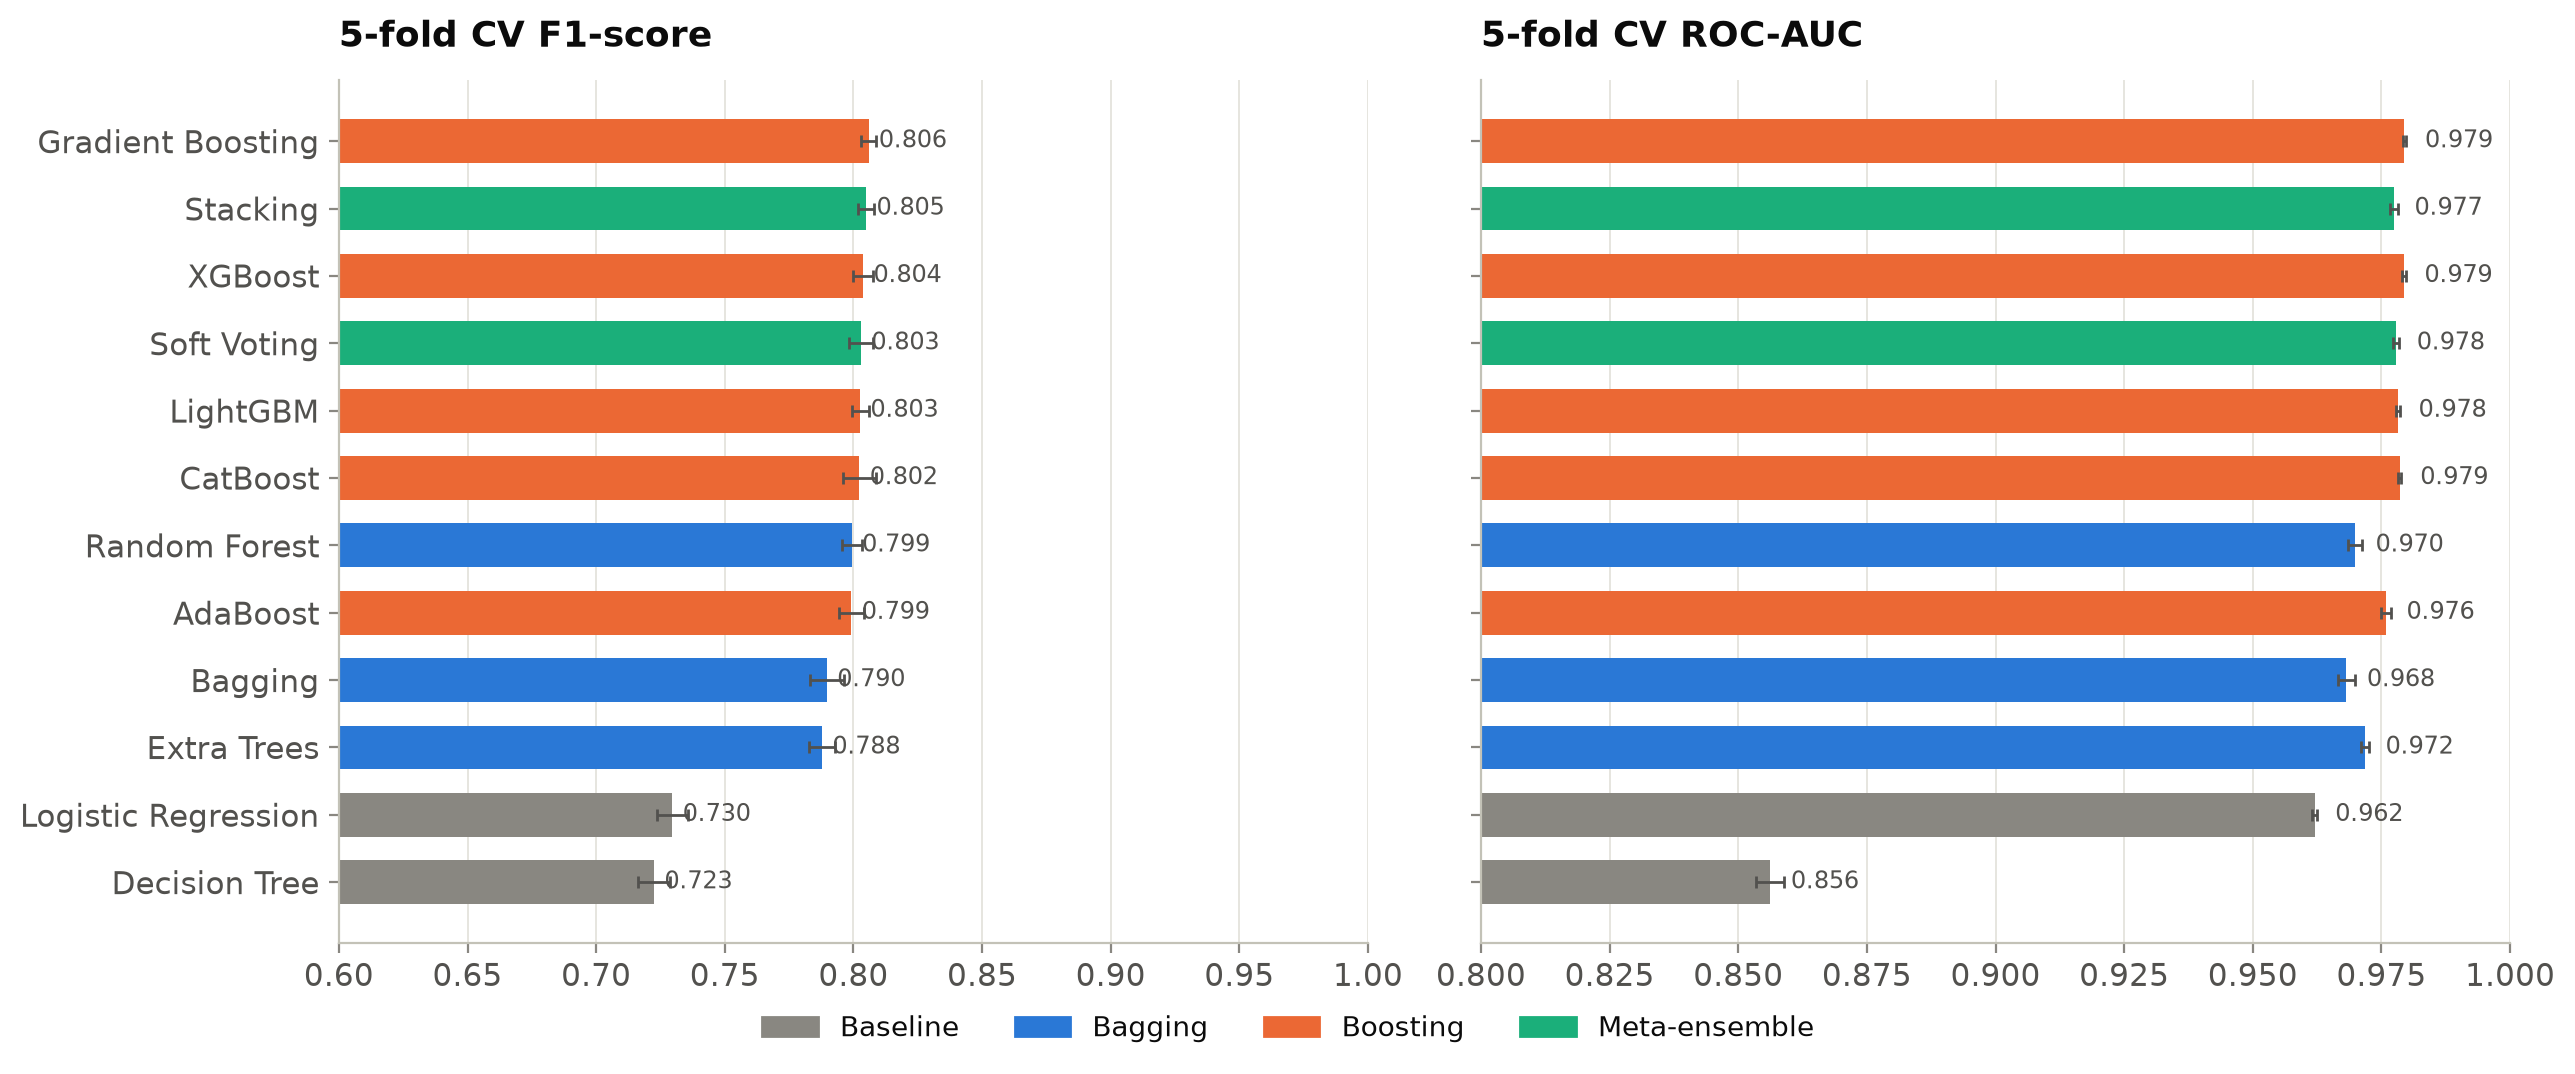
\includegraphics[width=\linewidth]{db_cv_comparison.png}
\caption{5-fold CV F1-score and ROC-AUC with standard deviation (grey = baselines, blue = bagging, orange = boosting, green = meta-ensembles)}
\label{fig:dbcv}
\end{figure}
\textbf{Interpretation (Table~\ref{tab:dbcv}, Figure~\ref{fig:dbcv}).} \DBCVINTERP

\begin{table}[H]
\centering
\caption{Held-out test set results at the default threshold 0.5 (sorted by F1)}
\label{tab:dbtest}
\begin{tabular}{@{}lccccccc@{}}
\toprule
\textbf{Model} & \textbf{Accuracy} & \textbf{Precision} & \textbf{Recall} & \textbf{F1} & \textbf{ROC-AUC} & \textbf{PR-AUC} & \textbf{Fit (s)} \\
\midrule
\dbTestRows
\bottomrule
\end{tabular}
\end{table}
\textbf{Interpretation (Table~\ref{tab:dbtest}).} \DBTESTINTERP

\begin{table}[H]
\centering
\caption{Test results with the F1-optimal threshold chosen on out-of-fold training predictions}
\label{tab:dbthr}
\begin{tabular}{@{}lcccccc@{}}
\toprule
\textbf{Model} & \textbf{Threshold} & \textbf{Accuracy} & \textbf{Precision} & \textbf{Recall} & \textbf{F1} & \textbf{ROC-AUC} \\
\midrule
\dbThrRows
\bottomrule
\end{tabular}
\end{table}
\textbf{Interpretation (Table~\ref{tab:dbthr}).} \DBTHRINTERP

\begin{figure}[H]
\centering
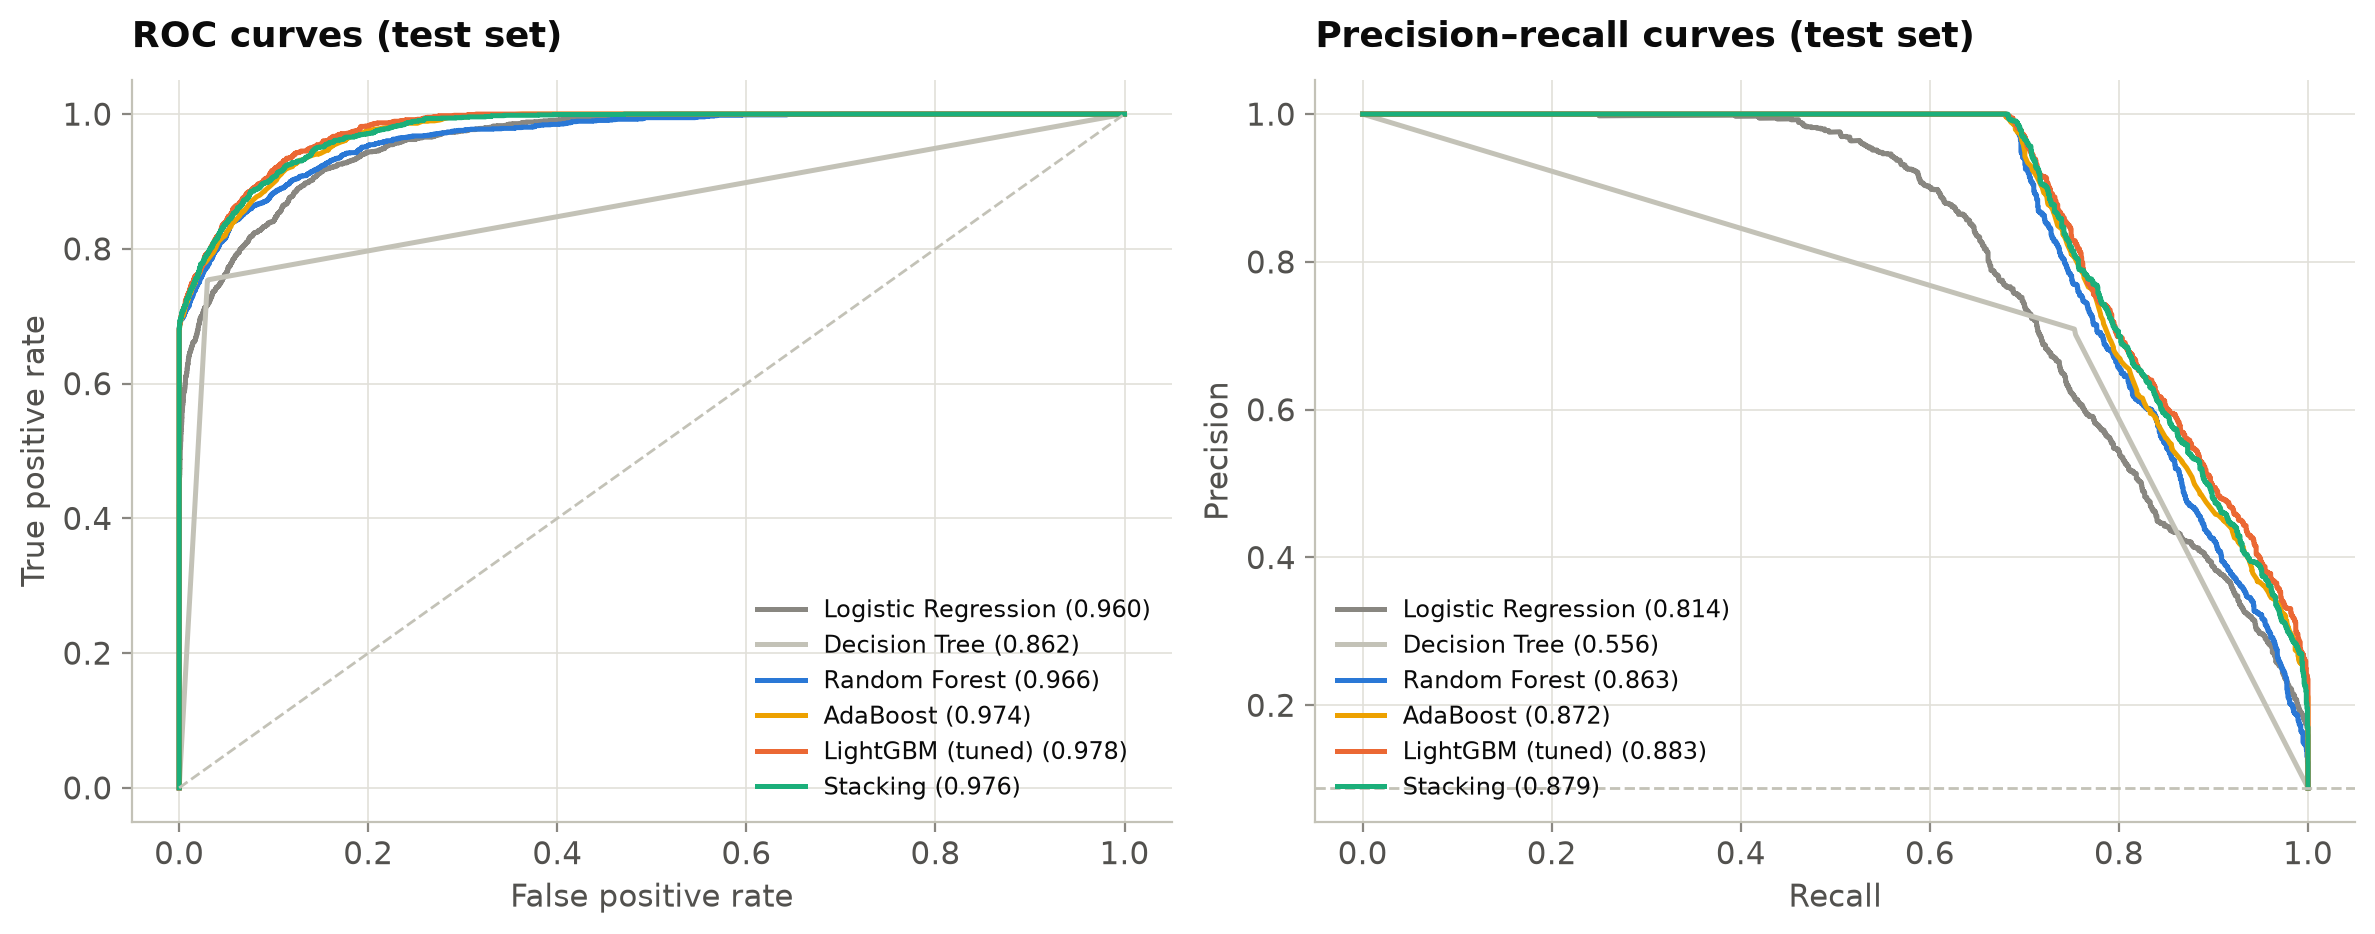
\includegraphics[width=\linewidth]{db_roc_pr.png}
\caption{ROC (left) and precision–recall (right) curves on the test set; AUC values in brackets}
\label{fig:dbroc}
\end{figure}
\textbf{Interpretation (Figure~\ref{fig:dbroc}).} \DBROCINTERP

\begin{figure}[H]
\centering
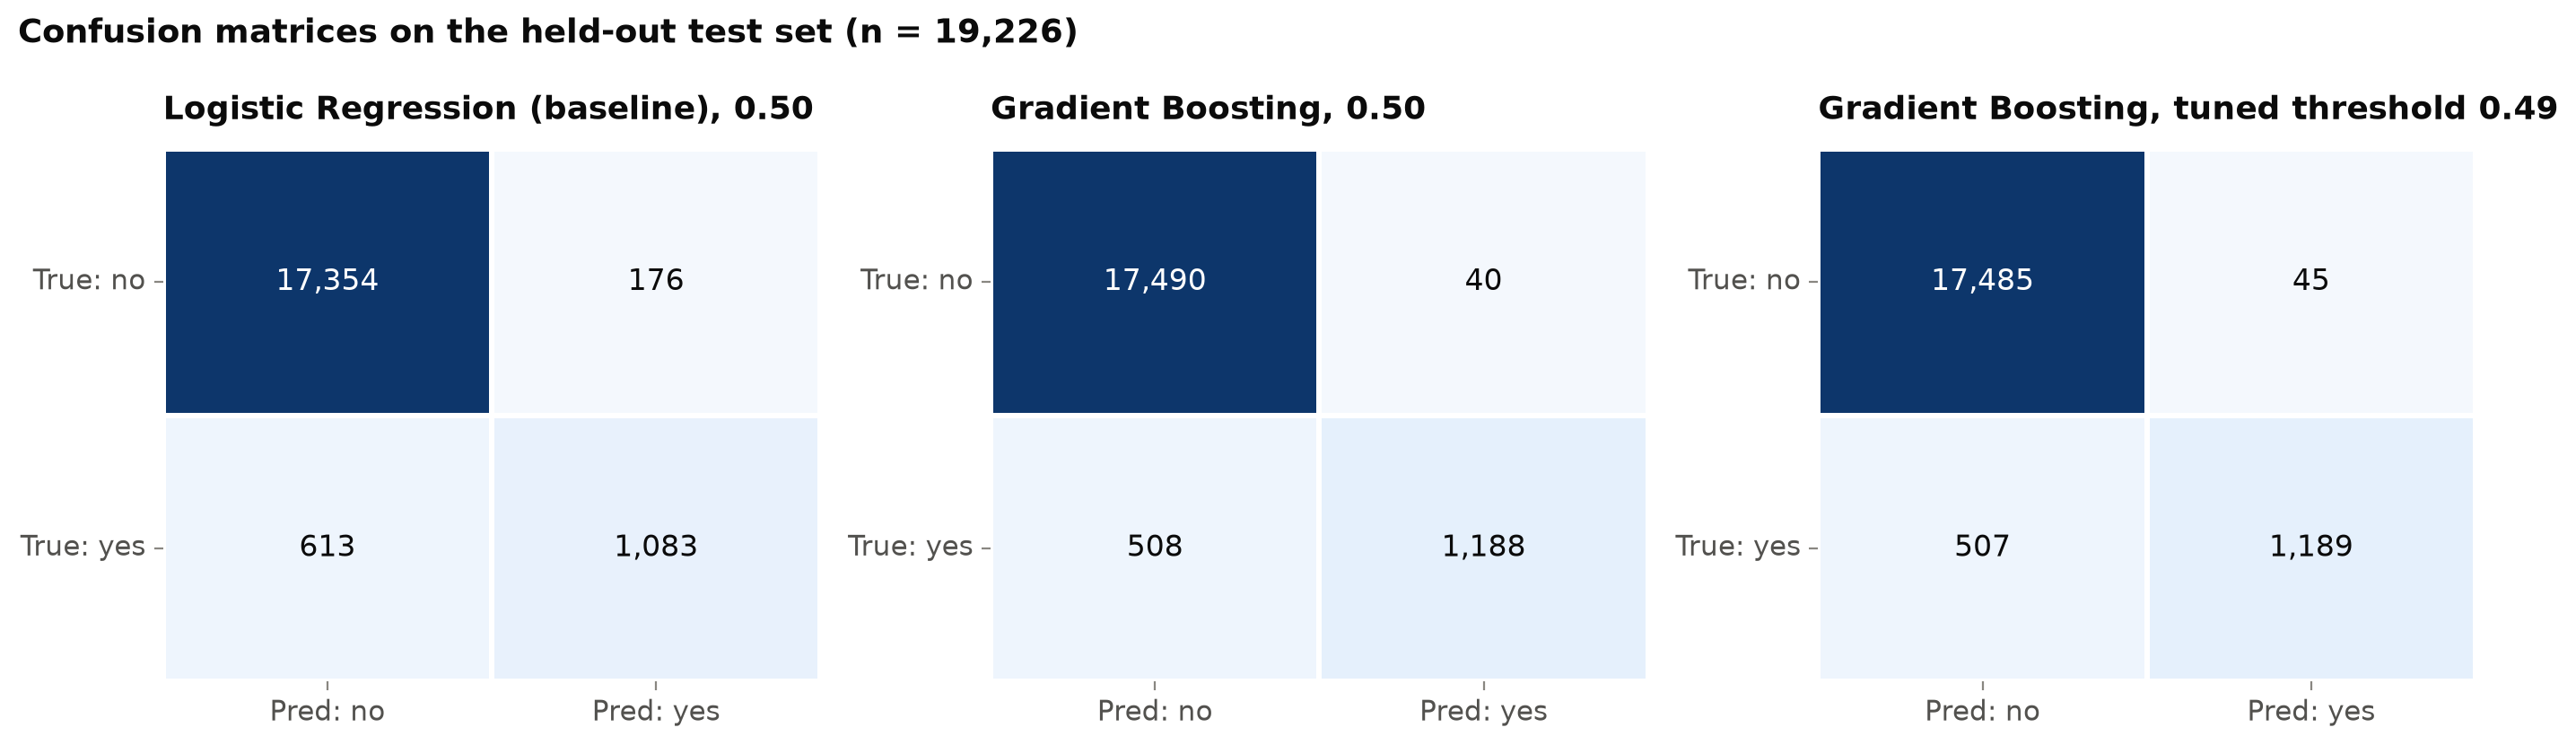
\includegraphics[width=\linewidth]{db_confusion.png}
\caption{Test-set confusion matrices: Logistic Regression baseline, best ensemble at 0.5, and best ensemble at the tuned threshold}
\label{fig:dbcm}
\end{figure}
\textbf{Interpretation (Figure~\ref{fig:dbcm}).} \DBCMINTERP

\begin{figure}[H]
\centering
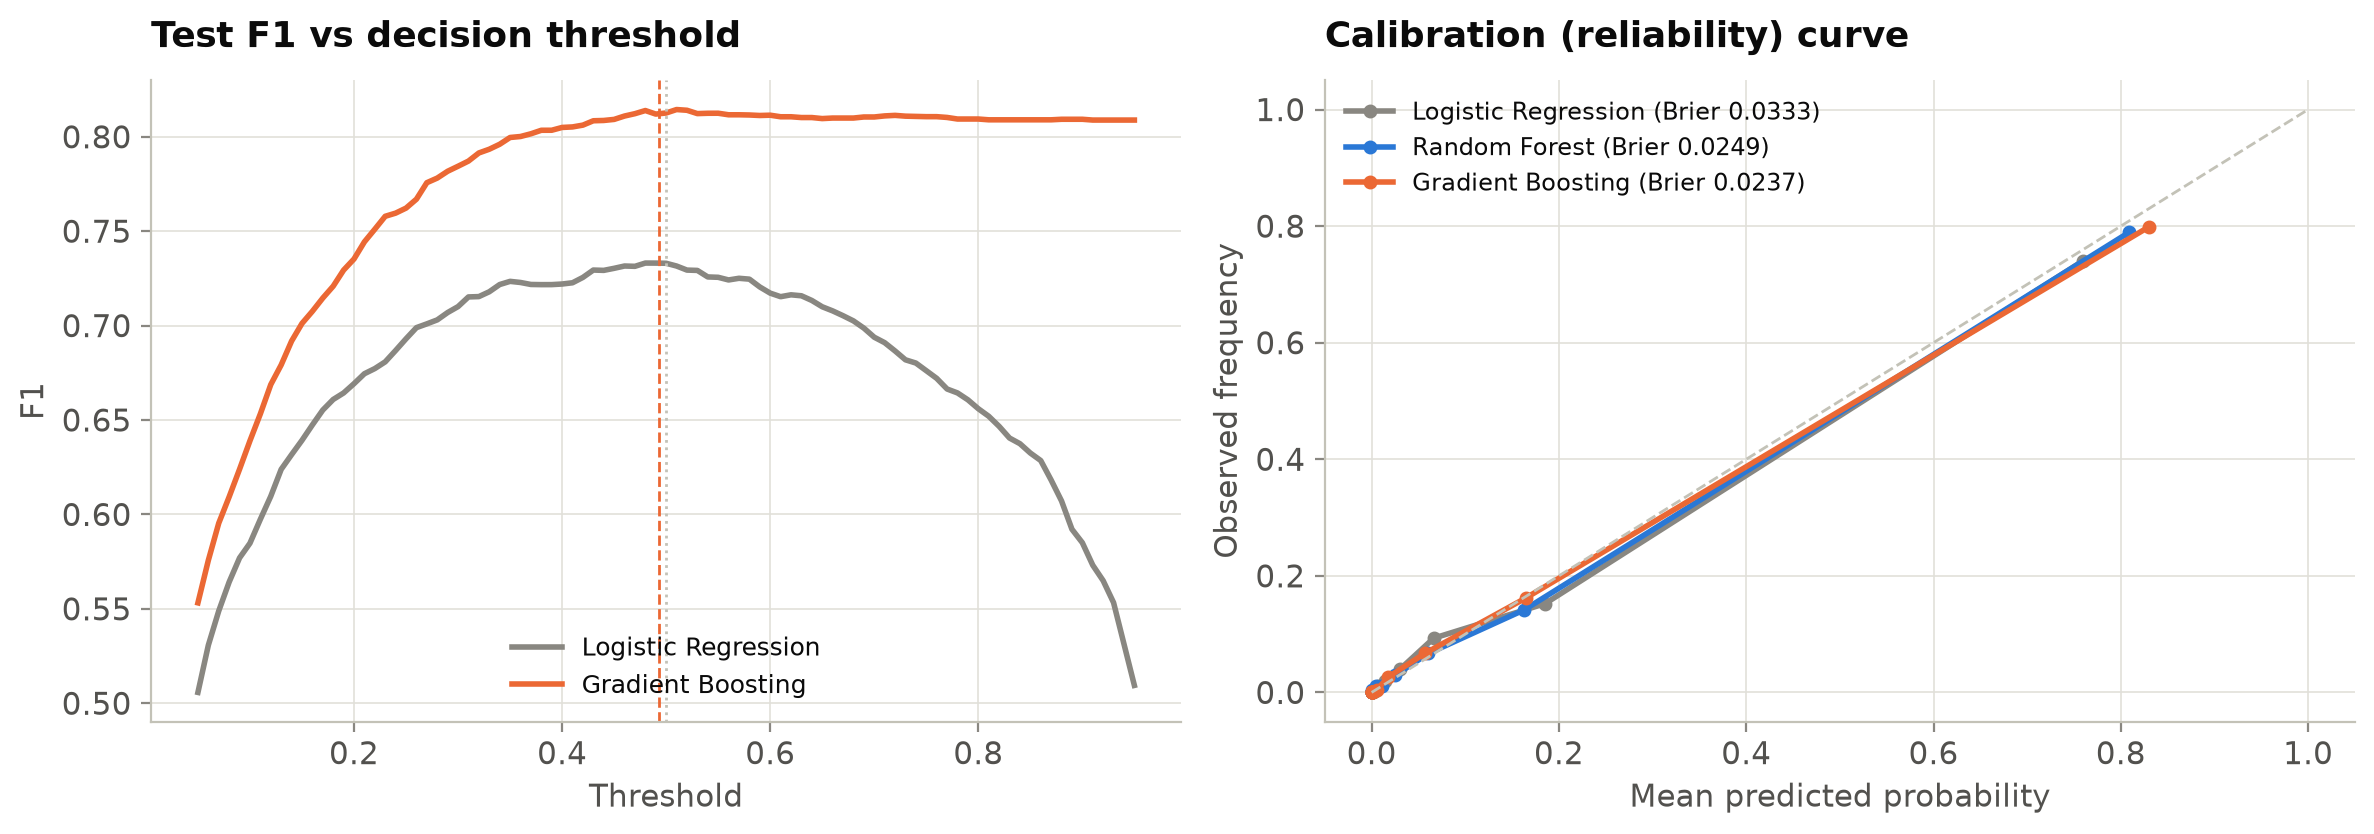
\includegraphics[width=\linewidth]{db_threshold_calibration.png}
\caption{Test F1 as a function of the decision threshold (left) and calibration curves (right)}
\label{fig:dbthr}
\end{figure}
\textbf{Interpretation (Figure~\ref{fig:dbthr}).} \DBTHRCALINTERP

\begin{figure}[H]
\centering
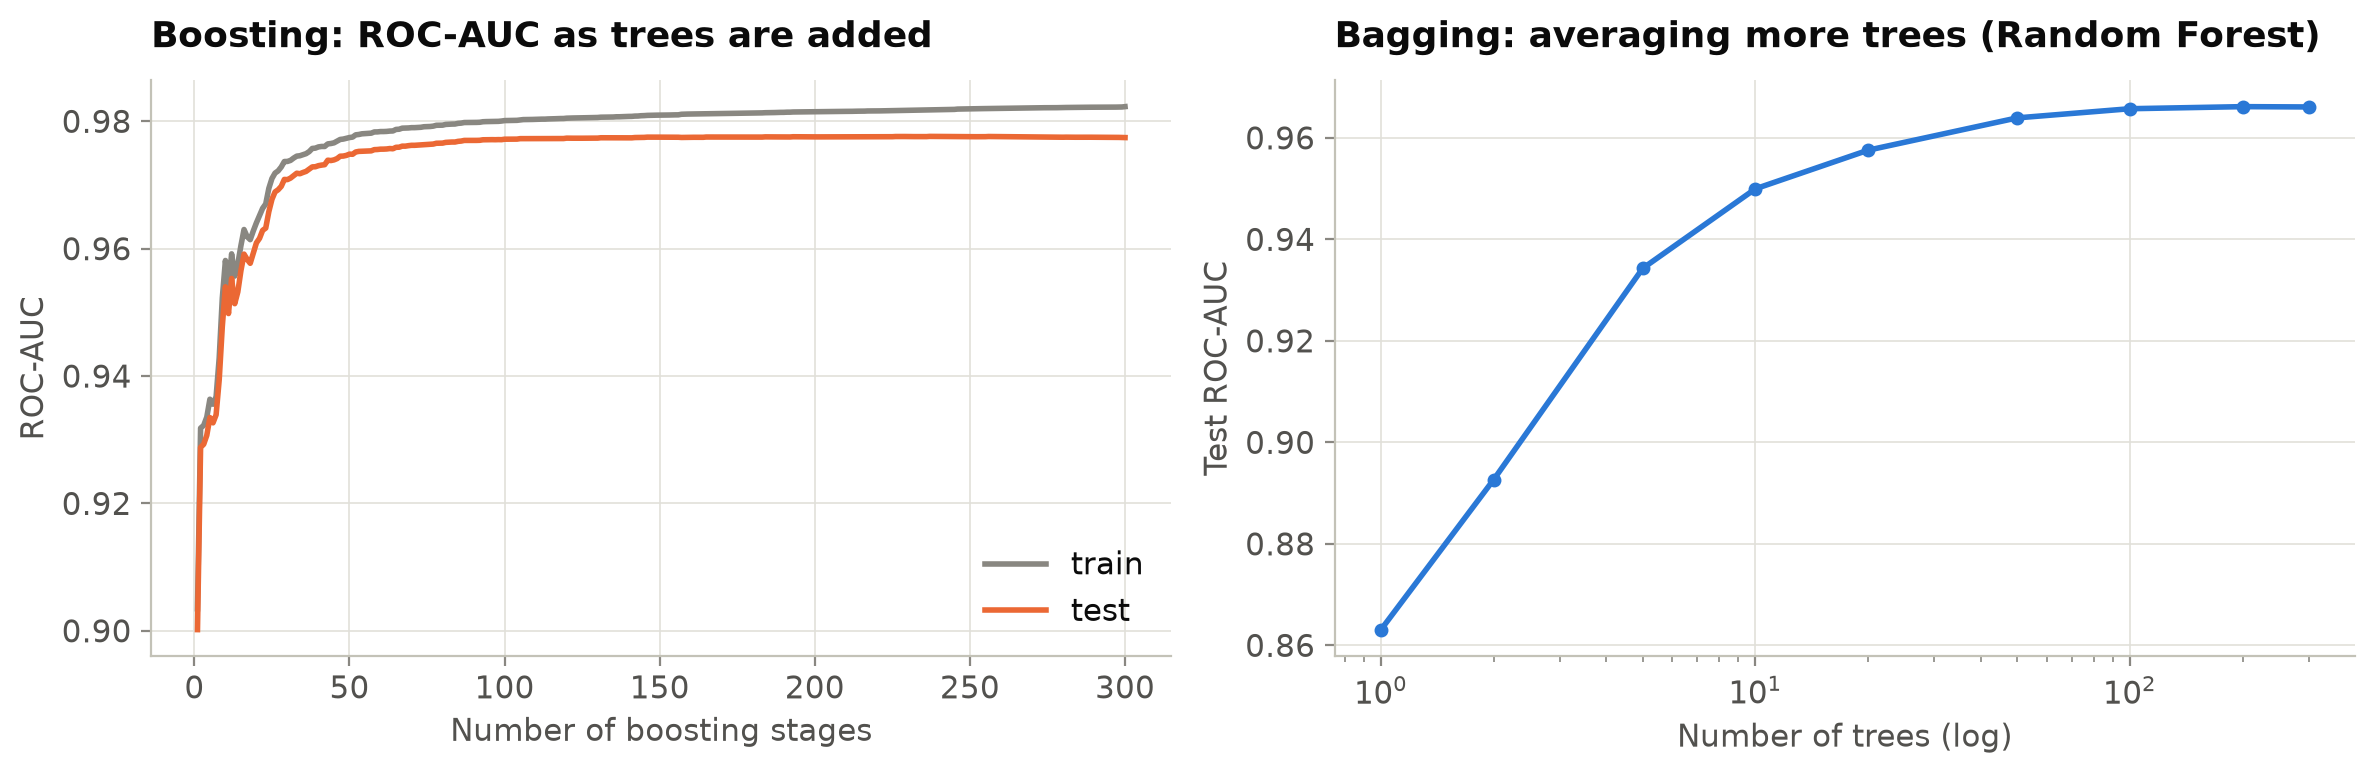
\includegraphics[width=\linewidth]{db_ensemble_size.png}
\caption{How ensembles improve: boosting ROC-AUC as trees are added (left); Random Forest test ROC-AUC vs number of averaged trees (right)}
\label{fig:dbsize}
\end{figure}
\textbf{Interpretation (Figure~\ref{fig:dbsize}).} \DBSIZEINTERP

\begin{table}[H]
\centering
\caption{Statistical significance: paired $t$-test on 5-fold CV F1 against Logistic Regression}
\label{tab:dbsig}
\begin{tabular}{@{}lcc@{}}
\toprule
\textbf{Model} & \textbf{Mean $\Delta$F1 vs LR} & \textbf{$p$-value} \\
\midrule
\dbSigRows
\bottomrule
\end{tabular}
\end{table}
\textbf{Interpretation (Table~\ref{tab:dbsig}).} \DBSIGINTERP

\begin{figure}[H]
\centering
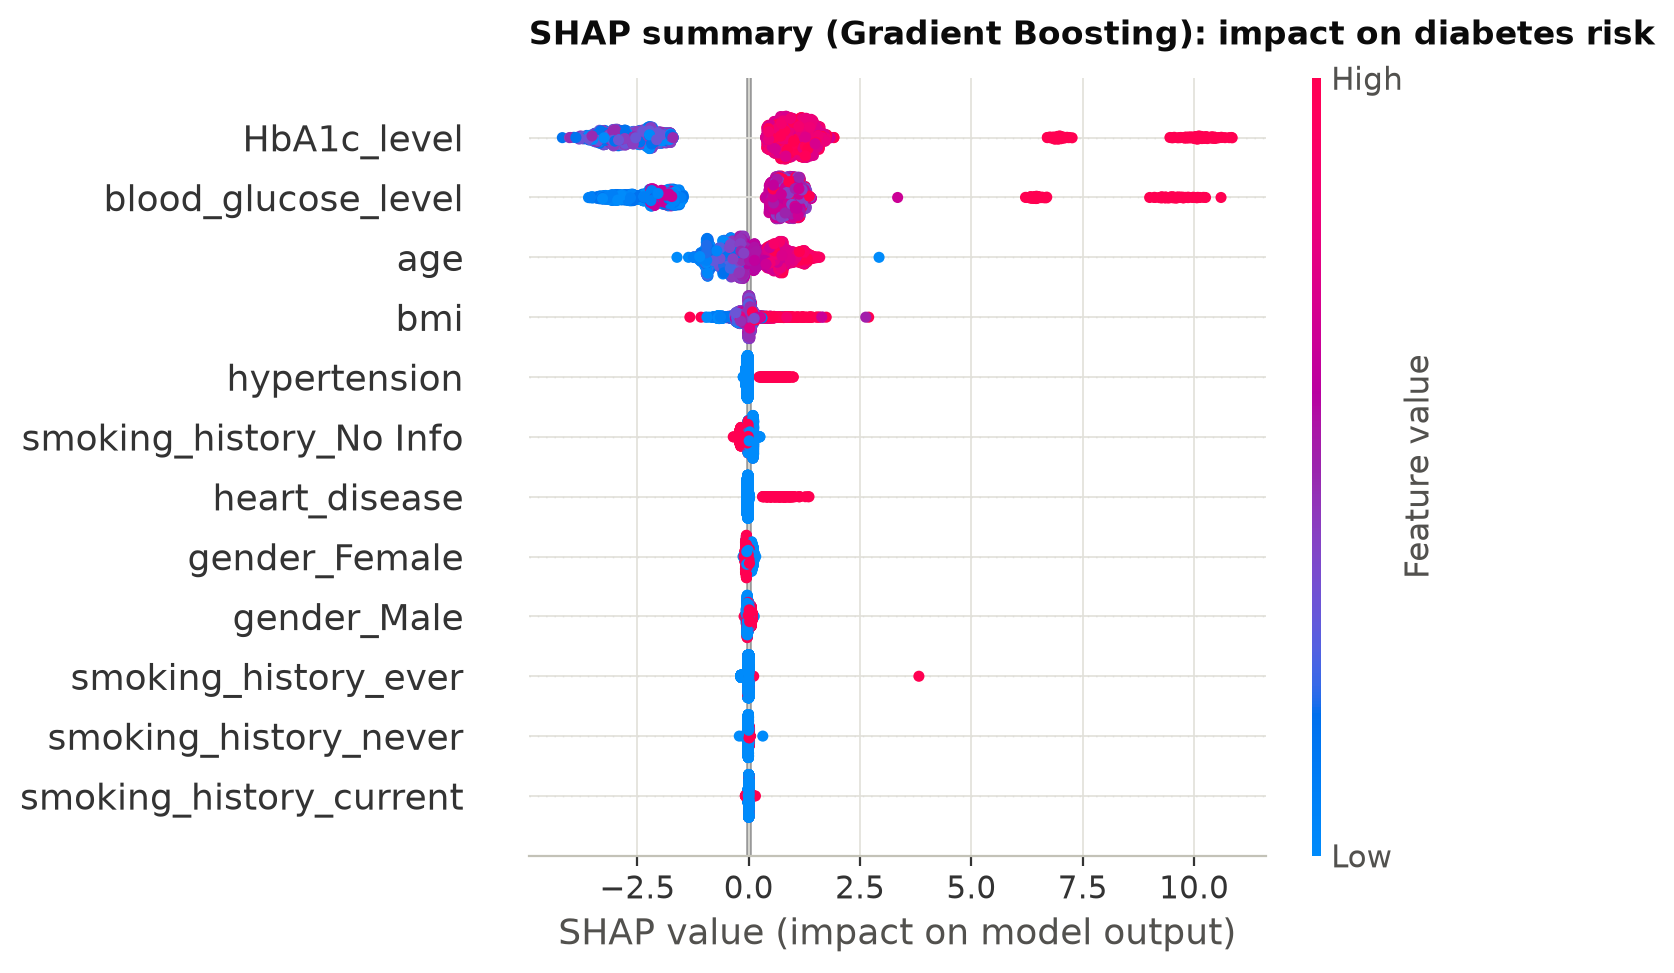
\includegraphics[width=0.56\linewidth]{db_shap_summary.png}\hfill
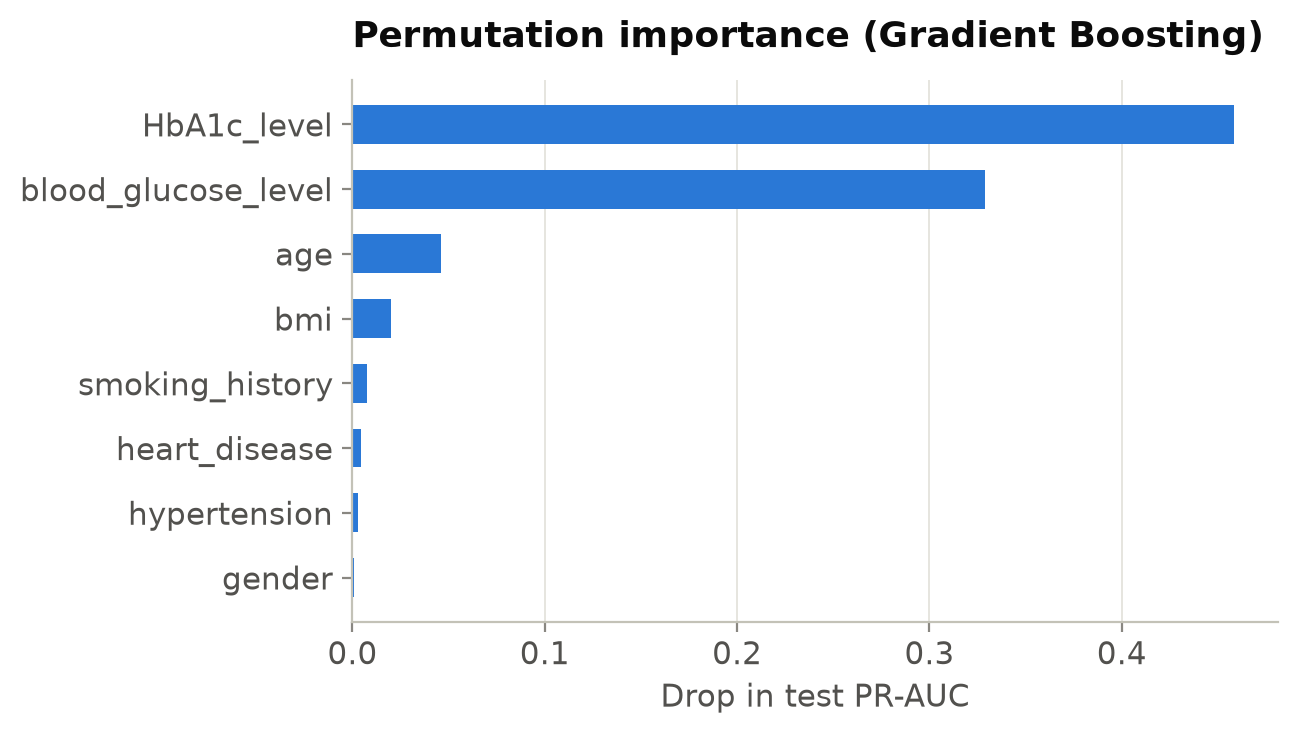
\includegraphics[width=0.42\linewidth]{db_permutation_importance.png}
\caption{SHAP summary for the final \dbShapModel{} model (left) and permutation importance on the test set (right)}
\label{fig:dbshap}
\end{figure}
\begin{figure}[H]
\centering
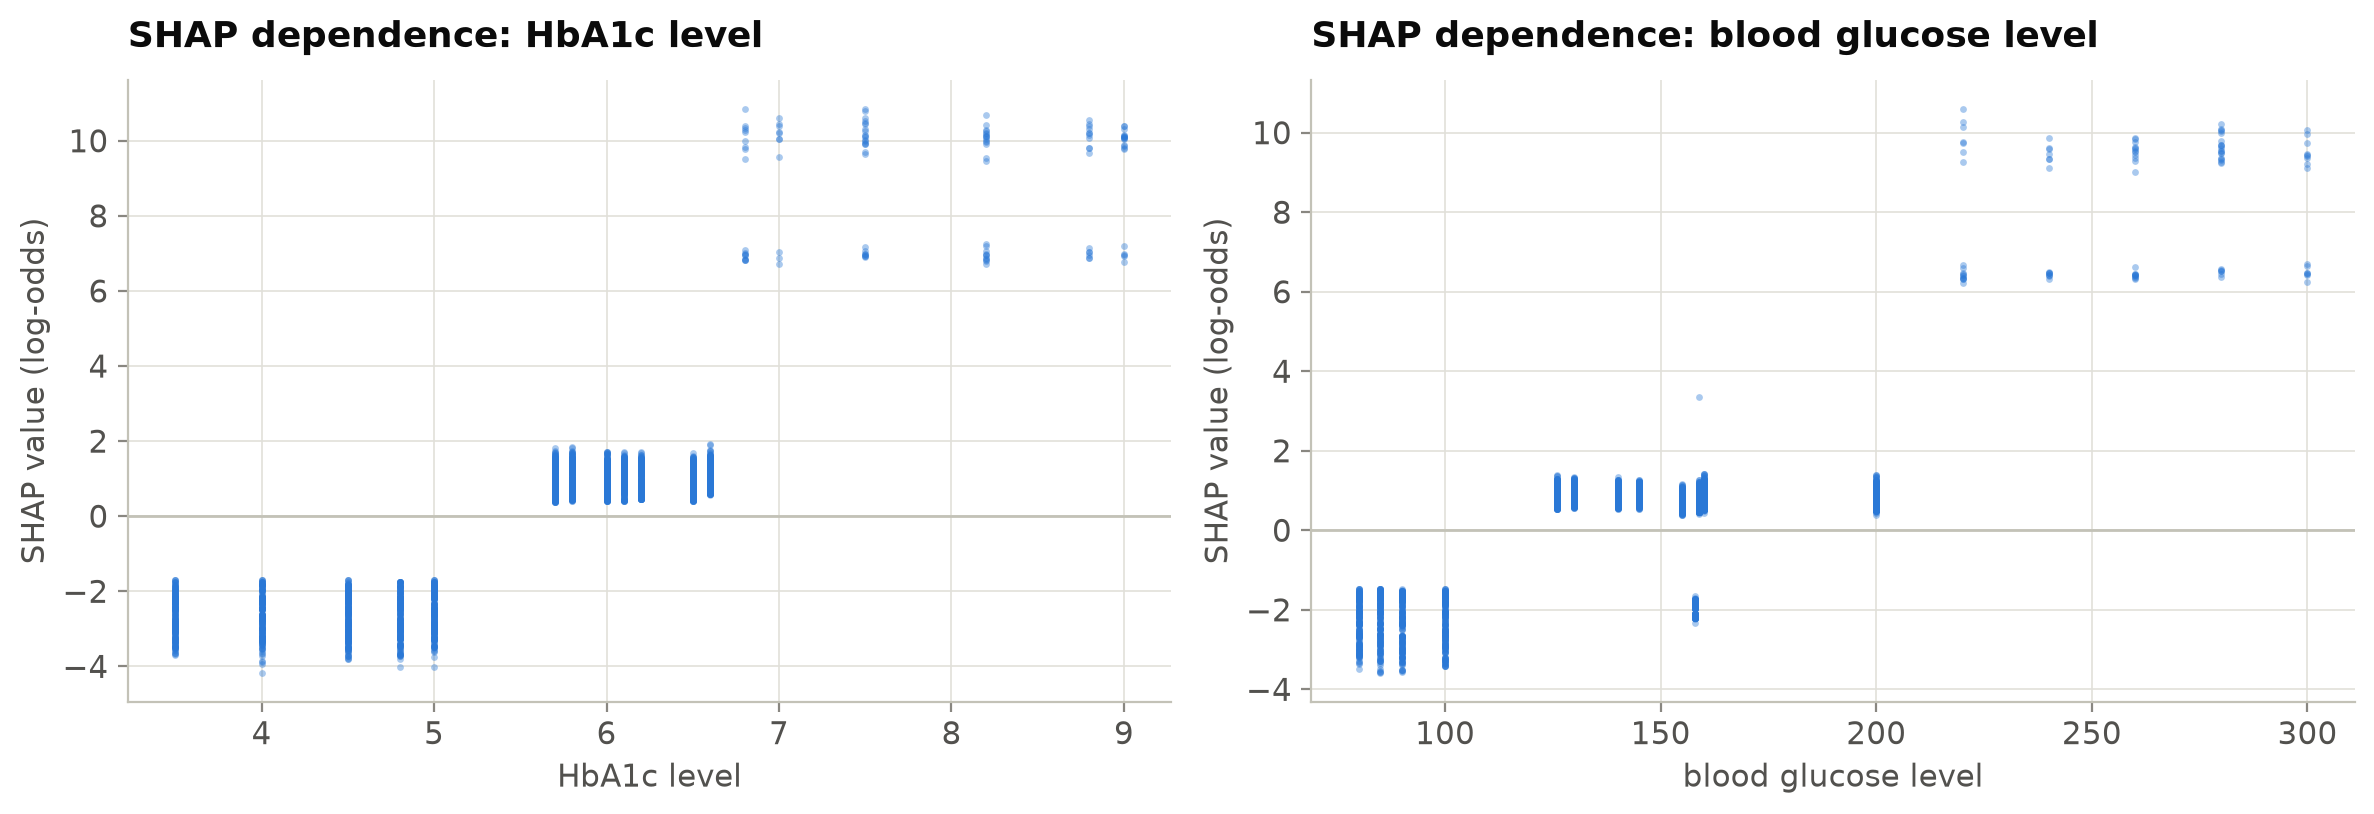
\includegraphics[width=\linewidth]{db_shap_dependence.png}
\caption{SHAP dependence of predicted risk on HbA1c and blood glucose}
\label{fig:dbshapdep}
\end{figure}
\textbf{Interpretation (Figures~\ref{fig:dbshap}–\ref{fig:dbshapdep}).} \DBSHAPINTERP

\section{Comparison with Previous Models}
\DBCOMPARE

\section{Discussion, Findings and Limitations}
\DBDISCUSS

\section{Chapter Conclusion}
\DBCONCL
